\section{Classical Capacity of Quantum Channels}

\subsection{Definition of Classical Capacity}
The classical capacity of a quantum channel \( \mathcal{N} \) is the maximum amount of classical information that can be transmitted per use of the channel with arbitrarily low error, as the number of channel uses goes to infinity. It is denoted by \( C(\mathcal{N}) \) and measured in bits per channel use.

\subsection{Types of Quantum Channels}
Quantum channels may be \textbf{noisy}, meaning they can alter or degrade the transmitted quantum states. Noise can arise from decoherence, loss, or other environmental factors. Common examples include depolarizing channels, dephasing channels, and amplitude-damping channels.

\begin{center}
    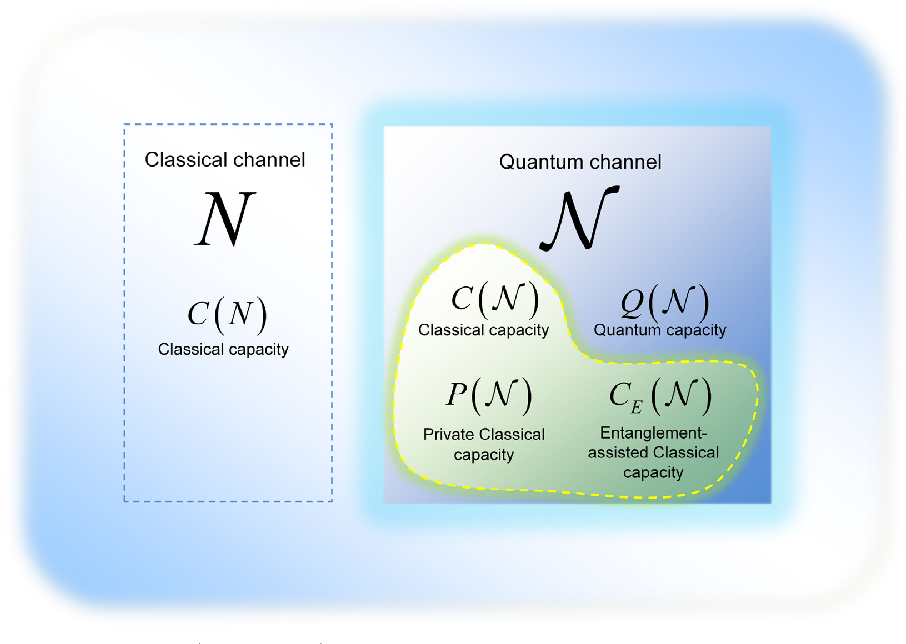
\includegraphics[width=0.5\textwidth]{figures/properties_channels.png}
\end{center}

\subsection{Formula for Classical Capacity}
The classical capacity \( C(\mathcal{N}) \) of a quantum channel \( \mathcal{N} \) is given by the regularized Holevo capacity:
\begin{equation}
    C(\mathcal{N}) = \lim_{n \to \infty} \frac{1}{n} \chi\left(\mathcal{N}^{\otimes n}\right)
\end{equation}
where \( \chi \) is the Holevo quantity, providing an upper bound on the amount of classical information that can be transmitted.

\begin{center}
    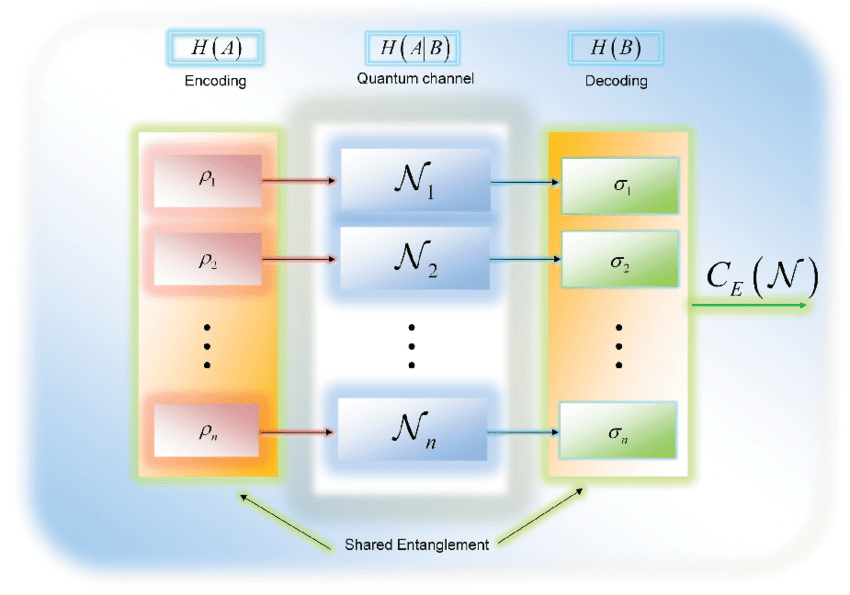
\includegraphics[width=0.75\textwidth]{figures/classical_cap.png}
\end{center}
\section{Citations for Images}

\begin{enumerate}
    \item \href{https://jahoo.github.io/2020/12/16/noisy-channel-coding.html}{Noisy Channel Coding - Jahoo Blog (2020)}
    \item \href{https://www.semanticscholar.org/paper/Properties-of-the-Quantum-Channel-Gyongyosi-Imre/0b473e0d1d4041ee6663691b5a96e8d6a5c82ba6/figure/34}{Properties of the Quantum Channel - Gyongyosi \& Imre, Semantic Scholar - Capacities of Classical and Quantum Channels (Figure 34)}

    \item \href{https://www.semanticscholar.org/paper/Properties-of-the-Quantum-Channel-Gyongyosi-Imre/0b473e0d1d4041ee6663691b5a96e8d6a5c82ba6/figure/15}{Properties of the Quantum Channel - Gyongyosi \& Imre, Semantic Scholar - Classical Capacity of a Quantum Channel (Figure 15)}
\end{enumerate}

